\section{Einleitung}\label{einleitung}

\subsection{Aufbau der Arbeit}\label{aufbau}
Nachdem einleitend der Aufbau der Bachelorthesis erläutert wird, baut das zweite Kapitel ein Grundverständnis zum Thema der Arbeit auf, indem Begriffsabgrenzungen und die Entwicklungen in Bezug auf das Thema aufgezeigt werden. Passend dazu werden die unterschiedlichen Channel-Arten aufbauend erklärt.
\newline
Im dritten Kapitel wird das Thema Omni-Channel untersucht und auf wichtige Faktoren zum erfolgreichen Umsetzen von Omni-Channel-Strategien eingegangen.
\newline
Für das vierte Kapitel, welches sich mit einer Analyse zur Umsetzung einer Omni-Channel-Strategie bei dem Unternehmen BABOR beschäftigt, wird unter anderem der Prozess zur Einführung eines neuen PIM-Systems näher beschrieben.
\newline
Zur weiteren Analyse folgen im fünften Kapitel das Ergebnis und die Handlungsempfehlung an Unternehmen, welche mit dem Gedanken spielen, die Kundenbedürfnisse tiefer in den Verkaufsprozess zu integrieren.
\newline
Zum Abschluss dieser Arbeit wird ein Fazit gezogen und ein Ausblick in die Zukunft gegeben.

\subsection{Problemstellung}\label{problemstellung}
Durch die Digitalisierung und der Entstehung neuer Technologien, wie \ac{zb} der Entwicklung der künstlichen Intelligenz, dem personalisiertem Einkaufserlebnis und damit weiteren Features wie dem Cross-Selling, entstanden in den letzten 10 Jahren für den elektronischen Handel ganz neue Verkaufs- und Vermarktungsmöglichkeiten, die sich noch immer schnelllebig weiterentwickeln. In Anbetracht steigender Ansprüche der Kunden und Kundinnen und der zunehmenden Innovationen im Bereich des Online-Vertriebs, hat es sich in den letzten Jahren zu einem Trend  entwickelt, dass Unternehmen ihre Vertriebswege erweitert haben und mittlerweile mehrere Vertriebskanäle managen müssen. Durch die Nutzung verschiedener Kanäle können Unternehmen hervorragende Wettbewerbsvorteile erzielen\footnote {Vgl. \autocite [S. 201] {Wirtz2013}}.
\newline

Wenn sich Konsumierende heutzutage für ein Beauty-Produkt interessieren, erwarten diese, dass ein Einstieg in den Kaufprozess zu jederzeit und überall möglich ist. Durch moderne Technologien und Geräte wie Smartphones und Tablets wird dies auch ermöglicht.
Die Herausforderung für den Handel ist, den Kundenbedürfnissen gerecht zu werden. Im Gegensatz zu den gewohnten Ladenöffnungszeiten, entstanden durch die permanente Verfügbarkeit der Online-Shops neue Möglichkeiten, die durch Weiterentwicklungen wie z.B. der SameDay-Delivery ausgebaut wurden. Diese neuen Meilensteine steigerten bei Konsumierenden die Kundenbedürfnisse. Aus Sicht der Unternehmen ist es ein Wettbewerbsvorteil, dass die Ansprüche der Konsumierenden erfüllt werden, um diese langfristig an sich binden zu können\footnote{Vgl. \autocite [Online] {walkersands2018}}.
\newline

Der Ausgangspunkt für Handelsstrategien war dabei der traditionelle Handel mit einer Single-Channel-Strategie, auf die im Verlauf näher eingegangen wird. Die Herausforderungen des elektronischen Handels führten zur Etablierung von Multi-Channel-Strategien. Heute verschmelzen die verschiedenen Verkaufskanäle durch den Multi-Channel-Commerce zu einem crossmedialen Dialog. Dabei spielt der Austausch mit Kunden und Kundinnen z.B. über Social Media Plattformen eine Rolle, aber vor allem auch ein auf die Konsumierenden zugeschnitteneres Einkaufserlebnis. Mit dem gleichzeitigen Anbieten von Produkten oder Marken über Social-Media wie Instagram oder Facebook wird durch einfache Feedbackmöglichkeiten auch die aktive Beteiligung der Kunden berücksichtigt.
\newline

Um das Online-Shopping überhaupt nutzen zu können, sind internetfähige mobile Endgeräte bei den Nutzer:innen notwendig. Die Verbreitung der Endgeräte ist in den letzten 10 Jahren explosionsartig gestiegen. Im Durchschnitt nutzten Ende 2021 in Deutschland 9 von 10 Personen im Alter von über 14 Jahren ein Smartphone und im Jahr 2020 besaß mehr als jede zweite Person ein Tablet\footnote{Vgl. \autocite [Online] {Touchpoints2022}}.
\begin{figure}[!ht]
    \centering
    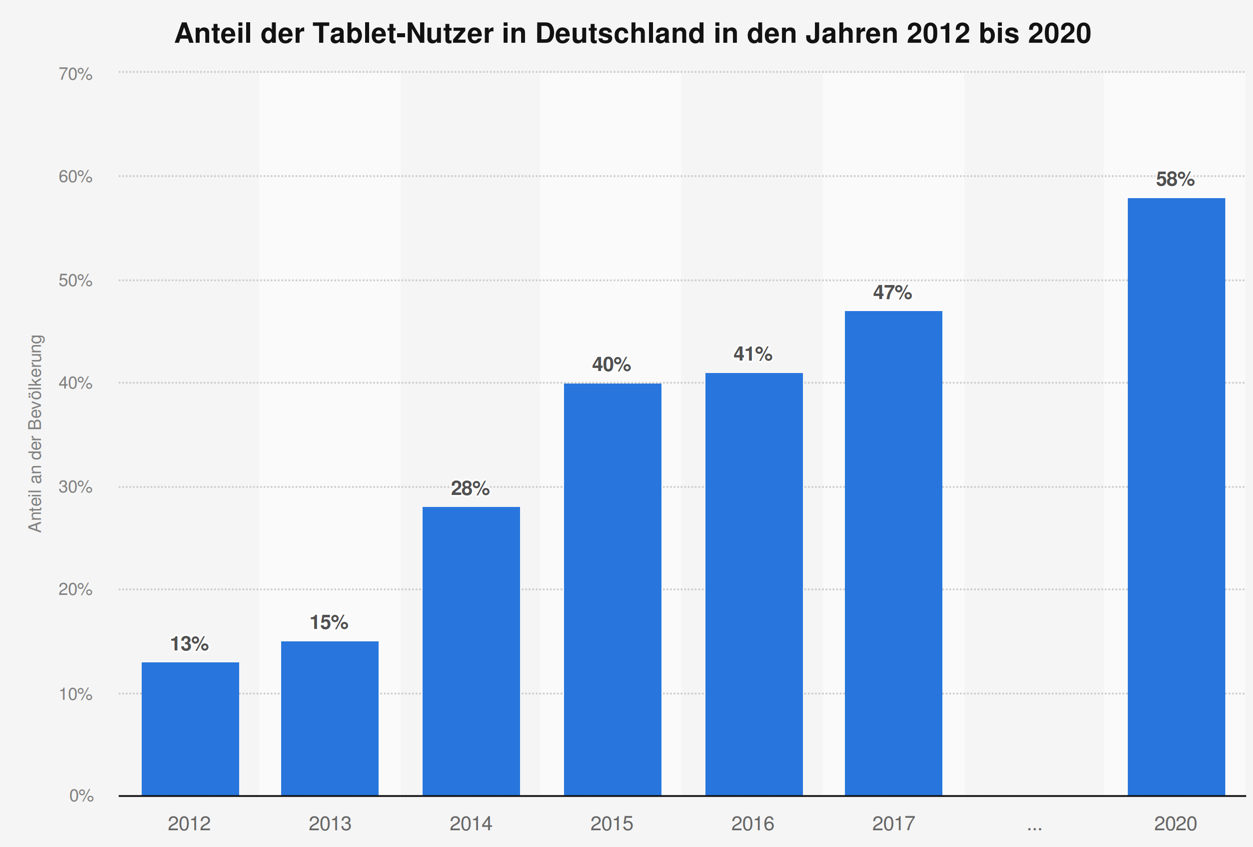
\includegraphics[width=1\textwidth,angle=0]{src/abbildungen/tabletnutzer_2020.png}
    \caption[Quelle: Bitkom, 2020]{Anteil der Tablet-Nutzer:innen in Deutschland von 2012 bis 2020, Quelle: \autocite {Bitkom2021}}
   \label{fig: tablet_nutzer}
   \end{figure}

Dabei zeigt sich, wie viel Potenzial im Online-Handel besteht, wenn ein Kosmetikunternehmen das Interesse potenzieller Kunden und Kundinnen mit Unterstützung einer nahtlosen Verknüpfung der Verkaufskanäle für sich gewinnen kann, wenn dadurch das Einkaufserlebnis kundennäher gestaltet wird. Der Kosmetikhandel kann von diesem Potenzial ebenfalls  profitieren, wenn die Konsumierenden durch richtige Strategieansätze angesprochen werden.

\subsection{Zielsetzung der Arbeit}\label{zielsetzung}
Ziel der Arbeit ist es, Informationen über die Wichtigkeit einer Omni-Channel-Strategie herauszuarbeiten und aufzuzeigen. Ergänzend dazu kann der Prozess zur Einführung eines PIM-Systems mit Hilfe einer Agentur näher beschrieben werden. Ein weiteres Ziel ist es dabei, die Anwendung einer beispielhaften Omni-Channel-Strategie aufzuzeigen.

\subsection{Vorgehensweise}\label{vorgehensweise}
Für die Bachelorthesis hat sich der Autor die folgende Forschungsfrage gestellt.
\newline
Welche spezifischen Herausforderungen und Chancen ergeben sich bei der Implementierung einer Omni-Channel-Strategie im Kosmetikbereich und wie wurden diese von dem Unternehmen BABOR gemeistert \asc{bzw} genutzt?
\newline

Durch Unterstützung von Literaturarbeit wurden zunächst die wichtigsten Punkte für die Anwendung und Umsetzung einer Omni-Channel-Strategie herausgesucht und analysiert. Dabei wurden Chancen und Herausforderungen von Omni-Channel-Strategien aufgedeckt und analysiert.